% !TeX root = ../../main.tex
\section{Detailed operating cost breakdown}
The following sections detail the annual operating expenditure (OPEX) incurred by Nitroma. The unit prices of all items were obtained from the negotiated price agreement with DEdwards Corp plc found in Section \ref{sec:price-agreement}. For all future OPEX projections, a cost escalation factor of \SI{2.6}{\percent} was applied to account for inflation in China (Statista 21). This is reflected on Nitroma’s financial statements in Section \ref{sec:economics-supporting}.

\subsection{Raw material cost}
\label{sec:opex-raw-material}

 \begin{table}[H]
\centering
\caption{OPEX: raw material}
\label{tab:Expansion}
\begin{tabular}{llll}
\toprule
\textbf{}      & \textbf{\begin{tabular}[c]{@{}l@{}}Unit price \\ (\$/kg)\end{tabular}} & \textbf{\begin{tabular}[c]{@{}l@{}}Quantity \\ (kg/year)\end{tabular}} & \textbf{\begin{tabular}[c]{@{}l@{}}Total cost \\ (\$)\end{tabular}} \\\midrule
Toluene        & 0.57                                                                   & 1,258,483                                                              & 717,335                                                             \\
Nitric acid    & 0.27                                                                   & 1,603,310                                                              & 432,894                                                             \\
Methanol       & 0.28                                                                   & 354,043                                                                & 99,132                                                              \\
Hydrogen       & 4.75                                                                   & 36,300                                                                 & 172,423                                                             \\
Formic acid    & 0.36                                                                   & 1,038,625                                                              & 373,905                                                             \\
\textbf{Total} & \textbf{}                                                              & \textbf{}                                                              & \textbf{1,795,689} \\\bottomrule                                                 
\end{tabular}
\end{table}

\subsection{Catalyst cost}
 The quantities of catalyst needed were estimated using detailed reactor modelling on COMSOL Multiphysics with a replacement frequency of 2 times per year (see Sections \ref{sec:detailedreactor} and \ref{Non-detailed}).

\begin{table}[H]
\centering
\caption{OPEX: Catalyst}
\label{tab:opex-catalyst}
\begin{tabular}{llll}
\toprule
\textbf{}                  & \textbf{Unit price (\$/kg)} & \textbf{Quantity (kg)} & \textbf{Total cost (\$)} \\ \midrule
H-Modernite                & 15.00                       & 118.00                 & 1,770                    \\
Palladium-on-carbon (5\%)  & 6,500.00                    & 27.42                  & 178,230                  \\
Cobalt (II) phthalocyanine & 12.00                       & 2,258.30               & 27,100                   \\
Platinum-on-carbon (5\%)   & 20,300.00                   & 344.90                 & 7,001,470                \\ 
\textbf{Total}             &                             &                        & \textbf{7,208,570}  \\\bottomrule    
\end{tabular}
\end{table}

\subsection{Utility cost}
 The quantities of cooling water and high-pressure steam were estimated using the heat duties of process units within the plant. Similarly, the electricity requirement was estimated by summing the power requirements of all process equipment.
 \begin{table}[H]
\centering
\caption{OPEX: Utilities}
\label{tab:opex-utilities}
\begin{tabular}{lllll}
\toprule
\textbf{}            & \textbf{Unit} & \textbf{Unit price} & \textbf{Quantity (unit/year)} & \textbf{Total cost (\$)} \\\midrule
Cooling water  (16C) & \$/tonne      & 0.26                & 930,563                       & 241,946                  \\
HP steam (4.3 MPa)   & \$/tonne      & 33.68               & 83,787                        & 2,821,950                \\
Electricity          & \$/kWh        & 0.104               & 11,280,192                    & 1,173,140                \\
\textbf{Total}       & \textbf{}     & \textbf{}           & \textbf{}                     & \textbf{4,237,036}      \\\bottomrule
\end{tabular}
\end{table}

\subsection{Labour cost}
As a continuous process, the plant must operate for 24 hours every day. Based on guidance from Towler \& Sinnott, three 8-hour shifts are planned, and five shift teams will be hired to account for weekends and holidays \cite{sinnott_chemical_2020}. Each shift team will be made up of 4 process operators (mixed solids-fluids processing) and 1 general foreman to overlook affairs within the team. 2 process engineers will be hired – one will be trained to oversee OTOL production and the other will be trained to oversee PABH production. Both share joint responsibility over PABA production. 2 quality engineers and 2 area supervisors will also be hired with the same breakdown of responsibilities.The area supervisors will report to 1 plant manager who will be responsible for overseeing the entire plant. A managerial support team of 6 admin staff will be hired with individual responsibilities including human resource management, finance, procurement, and sales. A team of 2 R\&D engineers will also be hired to prepare for 5-yearly plant expansions.
Table XX summarises Nitroma's labour costs. A \SI{12.4}{\percent} loading factor was applied to the total labour cost to account for pensions, health insurance and other employee benefits in China based on data from UHY (UHY 2021).

\begin{table}[H]
\centering
\caption{OPEX: Labour}
\label{tab:opex-labour}
\begin{tabular}{llll}
\toprule
\textbf{}        & \textbf{Total employees} & \textbf{Base salary (\$/year)}              & \textbf{Total salary (\$/year)} \\\midrule
Process operator & 20                       & 14,100.00                                   & 282,000.00                      \\
Process engineer & 2                        & 26,600.00                                   & 53,200.00                       \\
Quality engineer & 2                        & 27,200.00                                   & 54,400.00                       \\
Foreman          & 5                        & 28,200.00                                   & 141,000.00                      \\
Area supervisor  & 2                        & 31,300.00                                   & 62,600.00                       \\
R\&D engineer    & 2                        & 30,400.00                                   & 60,800.00                       \\
Plant manager    & 1                        & 45,500.00                                   & 45,500.00                       \\
Admin staff      & 6                        & 16,600.00                                   & 99,600.00                       \\
\textbf{Total}   & \textbf{40}              & \textbf{}                                   & \textbf{799,100.00}             \\
                 &                          & \multicolumn{1}{r}{\textit{12.4\% loading}} & \textbf{898,188.40} \\\bottomrule           
\end{tabular}
\end{table}

\subsection{Additional operating costs}
Table XX details additional costs incurred by Nitroma in operating the plant along with a brief note on the method of calculation, based on guidance from Towler \& Sinnott \cite{sinnott_chemical_2020}.

\begin{table}[H]
\centering
\caption{OPEX: Additional}
\label{tab:opex-add}
\begin{tabular}{l|ll}
\toprule
\textbf{Item}          & \textbf{Notes}                                                          & \textbf{Cost (\$/year)} \\
\midrule
Supervision            & This is taken to be 25\% of operating labour.                           & 224,547                 \\
Labour overheads       & This is taken to be 60\% of operating labour and supervision.           & 673,641                 \\
General plant overhead & This is taken to be 65\% of total labour, labour overheads              & 1,454,961               \\
                       & and maintenance. It includes corporate functions such as                &                         \\
                       & marketing, human resources and research \& development.                 &                         \\
Maintenance            & This is taken as 5\% of ISBL since there is solids handling   involved. & 442,024                 \\
Insurance              & This is taken to be 1\% of ISBL.                                        & 88,405                  \\
Depreciation           & This is determined by applying straight-line depcreiation to the        & 1,128,640               \\
                       & ISBL over the 20 year plant lifetime period, as guided by               &                         \\
                       & Coulson \& Richardson \cite{sinnott_coulson_2005}.                                             &                         \\
\textbf{Total}         & \textbf{}                                                               & \textbf{4,012,218}
\\\bottomrule
\end{tabular}
\end{table}

\begin{wrapfigure}{r}{8cm}
    \caption{OPEX Summary}
    \label{fig:OPEXSummary}
    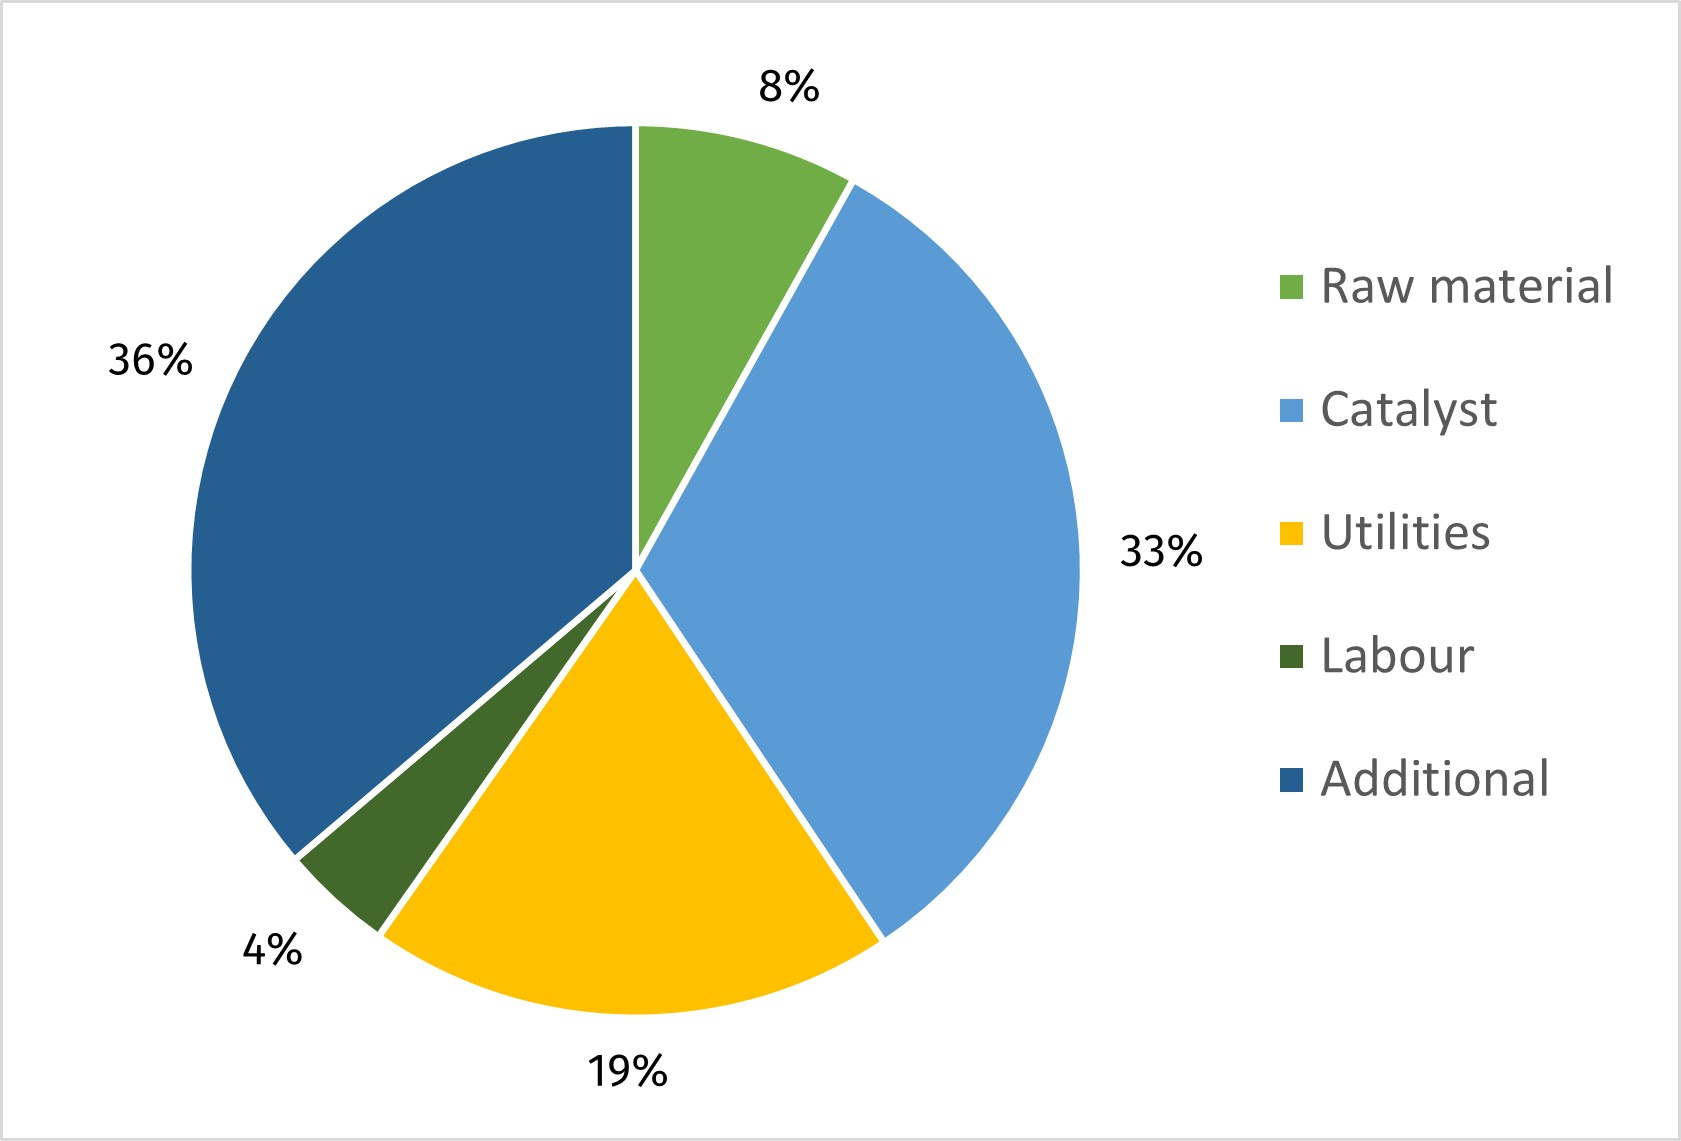
\includegraphics[width=0.47\textwidth]{chapters/6-economics/figures/OPEX_summary.jpg}
\end{wrapfigure}

\subsection{OPEX summary}

\begin{wrapfigure}{r}{8cm}
    \vspace{-1.1cm}
    \caption{OPEX Summary}
    \label{fig:OPEXSummary}
    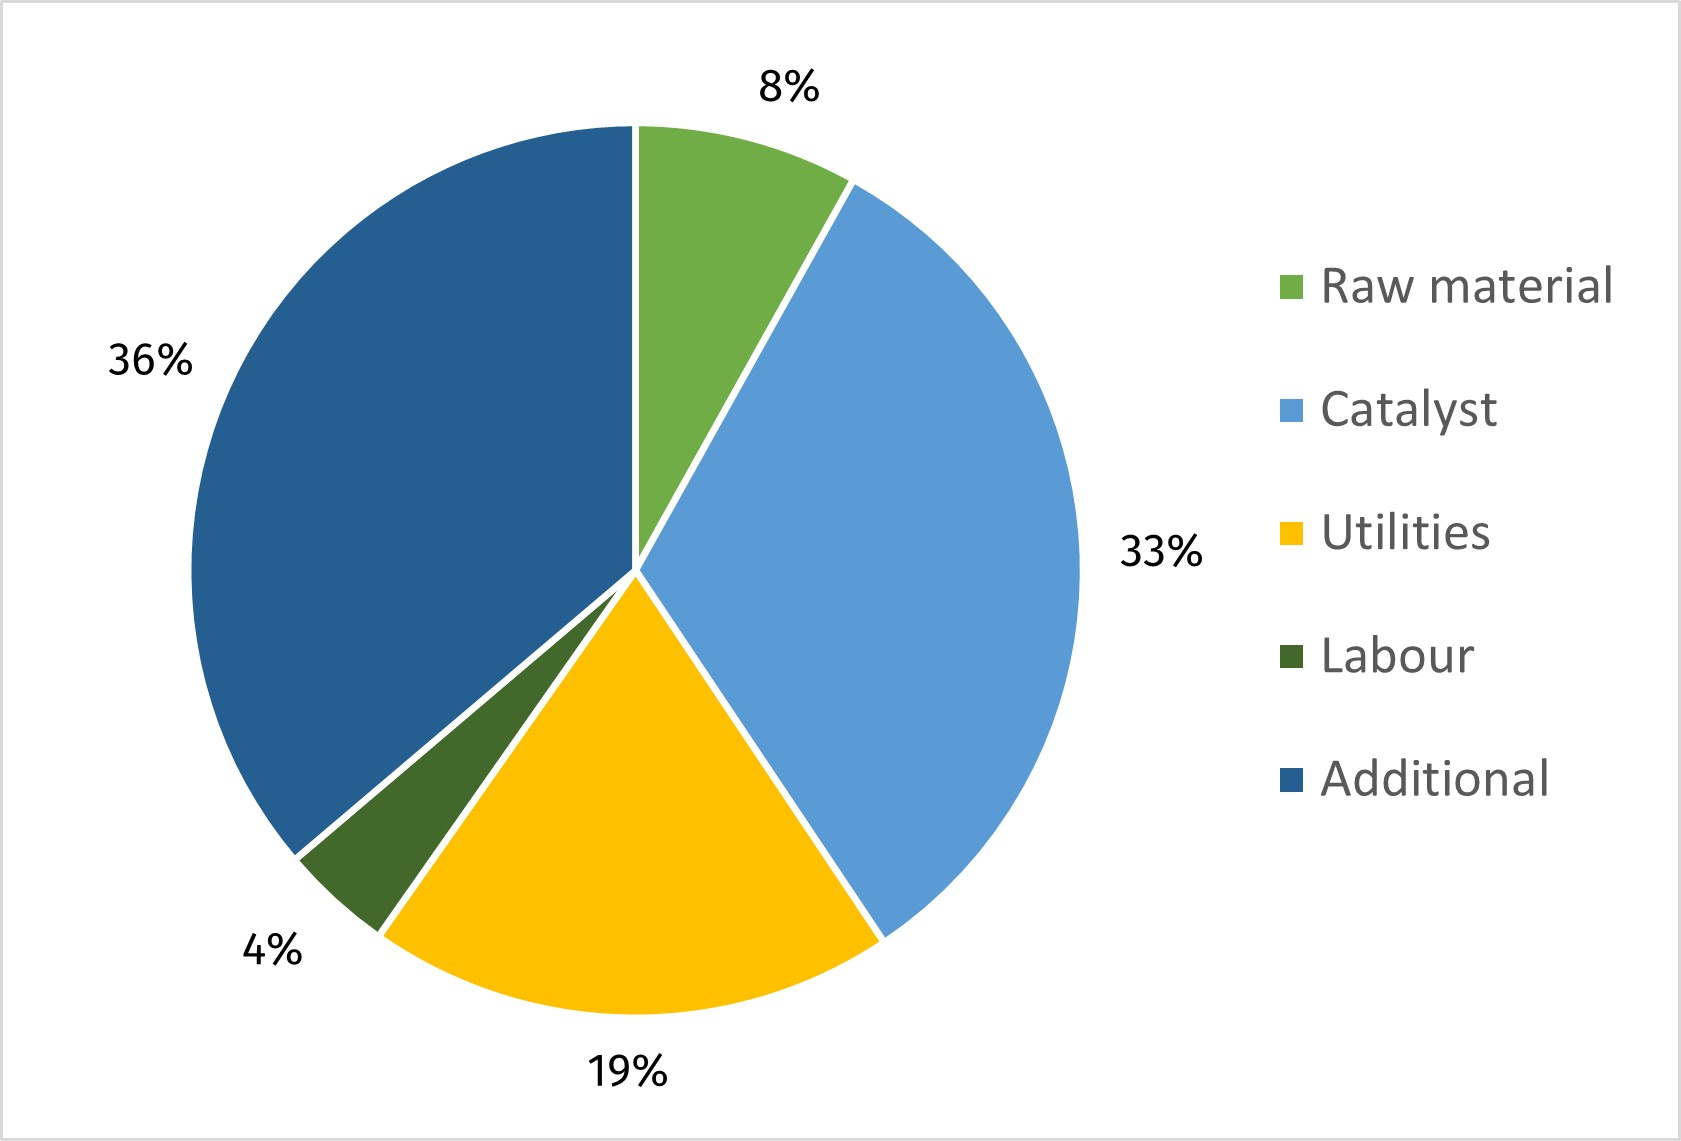
\includegraphics[width=0.47\textwidth]{chapters/6-economics/figures/OPEX_summary.jpg}
\end{wrapfigure}
The OPEX of the project was calculated to be \$18.2 million per annum based on current prices, comparatively lower than traditional batch nitration processes (general kinematics). A categorical breakdown of the OPEX can be seen in Figure XX. Moreover, Nitroma's cost of production was found to be \$15.81 per kg of output generated (detailed in Section \ref{sec:COP}), which is lesser than the speciality chemical industry average of \$24.54 per kg (maroulis 2016).